\documentclass{beamer}

\mode<presentation> 
{
    \usetheme{Madrid}
}

\usepackage[utf8x]{inputenc}
\usepackage[english,russian]{babel}
\usepackage[T2A]{fontenc}
\usepackage{graphicx}
\usepackage{booktabs} 
\usepackage{mathtools}
\usepackage{amsmath}
\usepackage{wasysym}
\usepackage{subfig}
\usepackage{hyperref}
\usepackage{ulem}
\usepackage{ragged2e}
\usepackage{algorithm2e}
\usepackage{minted}


\DeclarePairedDelimiter\ceil{\lceil}{\rceil}
\DeclarePairedDelimiter\floor{\lfloor}{\rfloor}


\usemintedstyle{borland}

\usefonttheme[onlymath]{serif}

\hypersetup
{
    colorlinks=true,
    linkcolor=white, 
    urlcolor=cyan
}

\title[Лекция 4]
{
    Лекция 4: Задача сортировка и функции в языке Си (продолжение)
} 


\author[Д. А. Караваев]{Д. А. Караваев}

\institute[СПбГУТ] 
{
    Санкт-Петербургский государственный университет телекоммуникаций \\ им. проф. М. А. Бонч-Бруевича \\ 
    \vspace{0.2cm}
    Факультет РТС, Кафедра РОС \\
    \vspace{0.2cm}
    Факультатив <<Программирование в ЦОС>> \\
    \vspace{0.2cm}
    Осень 2019
}

\date[11.11.2019]{11.11.2019 Санкт-Петербург} 

\begin{document}
    \begin{frame}
        \titlepage 
    \end{frame}
    \begin{frame}
        \frametitle{Аргументы функций}
        \justifying
        Существует два способа передачи аргументов в функцию:
        \begin{enumerate}
            \item {\bf По значению}: в качестве аргументов функции выступают соответствующие {\it копии} значений выражений, переданных в функцию в момент её вызова. Подобный механизм неявно реализован в Си (поведение по-умполчанию).
            \item {\bf По ссылке}: в качестве аргументов функции выступают {\it синонимы} переменных, переданных функцию. Подобный механизм используется в Java. В Си его можно реализовать явно при помощи {\it указателей}!
        \end{enumerate}
        \par
        {\bf Задача}: Что будет если мы захотим изменить значение той переменной, которая была передана в функцию в качестве параметра?
    \end{frame}
    \begin{frame}[fragile]
        \frametitle{Классический пример: функция {\tt swap}}
        \begin{minted}[frame=lines,         framesep=2mm,
                       baselinestretch=1.2, fontsize=\footnotesize,
                       linenos]{c}
/* Реализуем функцию, которая меняет значения двух переменных. */
/* Не правильно (оперируем с копиями, а не с самими перемнными): */
void swap_error(int x, int y)
{
    int temp = x;
    x = y;
    y = temp;
}
/* Правильно: используем указатели (передаём адреса, а не значения): */
void swap_correct(int* x, int* y)
{
    int temp = *x;
    *x = *y; /* (*x) - синоним переменной x! */
    *y = temp;
}
        \end{minted}
    \end{frame}
    \begin{frame}[fragile]
        \frametitle{Задача сортировки}
        \begin{block}{Формулировка}
            \justifying
            {\bf Вход}: Массив $a$ длины $N$;
            \par
            {\bf Выход}: Массив $a$ длины $N$: $a[0] \leq a[1] \leq \dotsc \leq a[N - 1]$ (по убыванию).
        \end{block}
        \par
        \begin{algorithm}[H]
            \DontPrintSemicolon
            \SetKwFunction{FSort}{InsertionSort}
            \SetKwFunction{FMinIndex}{MinIndex}
            \SetKwFunction{FSwap}{Swap}

            \SetKwProg{Fn}{Fuction}{:}{}
            \Fn{\FSort{$a$ : массив, $N$ : длина $a$}}
            {
                \For{$n \leftarrow 0$ \KwTo $N - 1$} 
                {
                    $j \leftarrow$ \FMinIndex($a,\ n,\ N$)\;
                    \FSwap($a[n],\ a[j]$)\;
                }
            }
            \;
            \Fn{\FMinIndex{$a$ : массив, $begin$ : начало, $end$ : конец}}
            {
                // Ваш (псевдо)код тут
            }
            \;
        \end{algorithm}
        \justifying
        \par
        {\bf Замечание}: Простейшим примером сортировки, является сортировка вставками (сложность $O(N^{2})$), основанная на поиске минимума.
    \end{frame}
    \begin{frame}
        \frametitle{Частный случай}
        \justifying
        {\bf Посылка}: Представим, что правая и левая половины $a$ отсортированы в нужном порядке:
        $$mid = \floor*{\frac{N}{2}},$$
        $$a[0\dotsc  mid - 1]:\ a[0] \leq \dotsc \leq a[mid - 1],$$
        $$a[mid \dotsc N - 1]:\ a[mid] \leq \dotsc \leq a[N - 1].$$
        \par
        \vspace{0.2cm}
        \justifying
        {\bf Задача}: Как получить ({\it слить}) остортированный массив $a$ на основе двух его отсортированных половин?
    \end{frame}
    \begin{frame}[fragile]
        \frametitle{Процедура слияния}
        \begin{algorithm}[H]
            \DontPrintSemicolon
            \SetKwFunction{FMerge}{Merge}

            \SetKwProg{Fn}{Fuction}{:}{}
            \Fn{\FMerge{$a, begin, mid, end$}}
            {
                $n_{1} \leftarrow mid - begin,\ n_{2} \leftarrow end - mid,\ L[n_{1} + 1],\ R[n_{2} + 1]$\;
                \For{$i \leftarrow 0$ \KwTo $n_{1} - 1$} 
                {
                    $L[i] \leftarrow a[begin + i]$\;
                }
                \For{$j \leftarrow 0$ \KwTo $n_{2} - 1$} 
                {
                    $R[j] \leftarrow a[mid + j]$\;
                }
                $L[n_{1}] \leftarrow \infty,\ R[n_{2}] \leftarrow \infty,\ i \leftarrow 0,\ j \leftarrow 0$\;
                \For{$k \leftarrow begin$ \KwTo $end - 1$} 
                {
                    \eIf{$L[i] \leq R[j]$}
                    {
                        $a[k] \leftarrow L[i],\ i \leftarrow i + 1$\;
                    }
                    {
                        $a[k] \leftarrow R[j],\ j \leftarrow j + 1$\;
                    }
                }
            }
        \end{algorithm}
    \end{frame}
    \begin{frame}[fragile]
        \frametitle{Сортировка слиянием}
        \justifying
        {\bf Рекурсивный переход}: Когда $a$ состоит из двух элементов, то обе его части отсортированы (начальное условие).
        \par
        {\it Cледовательно, рекурсивно разбивая массив на части до единичных элементов, можно отсортировать массив, применяя процедуру слияния для каждого этапа разбиения}.
        \par
        \vspace{0.5cm}
        \begin{algorithm}[H]
            \DontPrintSemicolon
            \SetKwFunction{FMergeSort}{MergeSort}

            \SetKwProg{Fn}{Fuction}{:}{}
            \Fn{\FMergeSort{$a$ : массив, $begin$ : начало, $end$ : конец}}
            {
                \If{$(end - begin) \neq 1$}
                {
                    $mid = \floor*{\frac{begin + end}{2}}$\; 
                    \FMergeSort($a, begin, mid$)\;
                    \FMergeSort($a, mid, end$)\;
                }
            }
        \end{algorithm}
        \par
        \vspace{0.5cm}
        \justifying
        {\bf Сложность}: Временная $\Theta(N \log_{2}{N})$, {\it пространственная}: $\Theta(N)$.
    \end{frame}
    \begin{frame}
        \frametitle{Иллюстрация сортировки слиянием}
        \begin{figure}[!tbp]
           \centering
           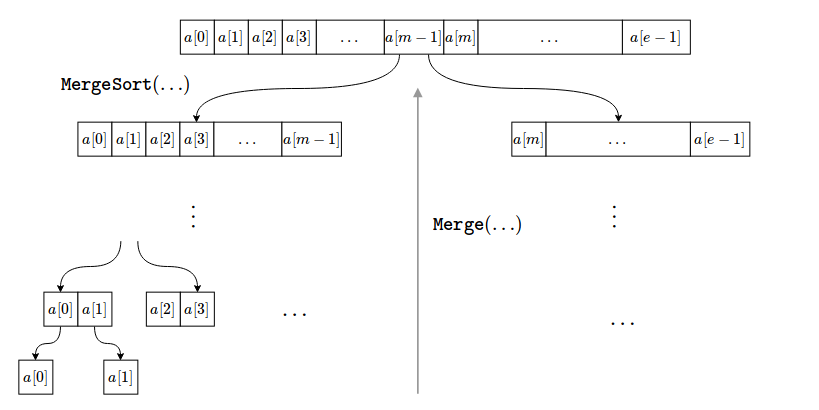
\includegraphics[width=\textwidth]{pics/sort.png}
       \end{figure}
    \end{frame}
    \begin{frame}
        \frametitle{Другие виды сортировок}
        \begin{enumerate}
            \justifying
            \item {\bf Быстрая сортировка*}: Временная сложность в среднем $O(N\log_{2}{N})$, память - in-place;
            \item {\bf Пирамидальная сортировка}: Временная сложность $O(N\log_{2}{N})$, память - in-place (основана на структуре данных - пирамида);
            \item {\bf Подсчётом}:  Временная сложность $\Theta(k)$, где $k$ - максимально возможное значение элемента, память -  $\Theta(k)$;
            \item {\bf Сортровка пузырьком}:  Временная сложность $O(N^{2})$,  память - in-place.
        \end{enumerate}
    \end{frame}
    \begin{frame}[fragile]
        \frametitle{Задания}
        \justifying
        В файле проекта {\tt Sort/source/main.c}
        \begin{enumerate}
            \item Реализовать сортировку вставками (3 процедуры);
            \item Реализовать сортировку слиянием (2 процедуры).
        \end{enumerate}
        \vspace{1cm}
        \par
        \justifying
        {\bf Замечание}: Для сборки используйте те же команды, что и для прокетов {\tt Convolution} и {\tt Search}. Для проверки результатов воспользуйтесь функцией {\tt printf(...)}.
    \end{frame}
    \begin{frame}
        \begin{center}
        \baselineskip 20.0mm
        \Huge Спасибо за внимание!
        \end{center}
    \end{frame}
\end{document}
